\chapter{Kekekalan Massa dan Persamaan Reaksi Setara}\label{ch:g8:balanced-equations}

Sebatang kayu gelondongan seberat dua kilogram \omterm{def:g4:what-a-fire-needs:burning}{terbakar} di perapian.
Pagi harinya, yang tersisa hanya beberapa puluh gram abu kelabu. Apakah
hampir dua kilogram materi lenyap dalam semalam? Selama berabad-abad
tidak seorang pun dapat menjawabnya. Jawabannya datang dari seorang ahli
kimia yang memutuskan untuk menimbang segalanya --- termasuk gas-gas
yang tidak pernah terpikirkan untuk ditimbang orang.

\begin{recall}
Dalam \omterm{def:g7:chemical-reactions:reaction}{reaksi kimia}, \omterm{def:g7:chemical-reactions:reactant}{pereaksi} terpakai dan produk terbentuk; \omterm{def:g7:atoms-and-molecules:atom}{atom-atom}
\omterm{def:g7:chemical-reactions:reactant}{pereaksi} ditata ulang menjadi produk, tidak diciptakan dan tidak
dimusnahkan (\cref{ch:g7:chemical-reactions}). \omterm{def:g7:atoms-and-molecules:formula}{Rumus kimia} seperti
\ce{H2O} mendaftar \omterm{def:g7:atoms-and-molecules:atom}{atom-atom} sebuah \omterm{def:g7:atoms-and-molecules:molecule}{molekul}; angka di depannya, seperti
pada \ce{3H2O}, menghitung \omterm{def:g7:atoms-and-molecules:molecule}{molekul} (\cref{ch:g7:atoms-and-molecules}).
\end{recall}

\begin{omfigure}
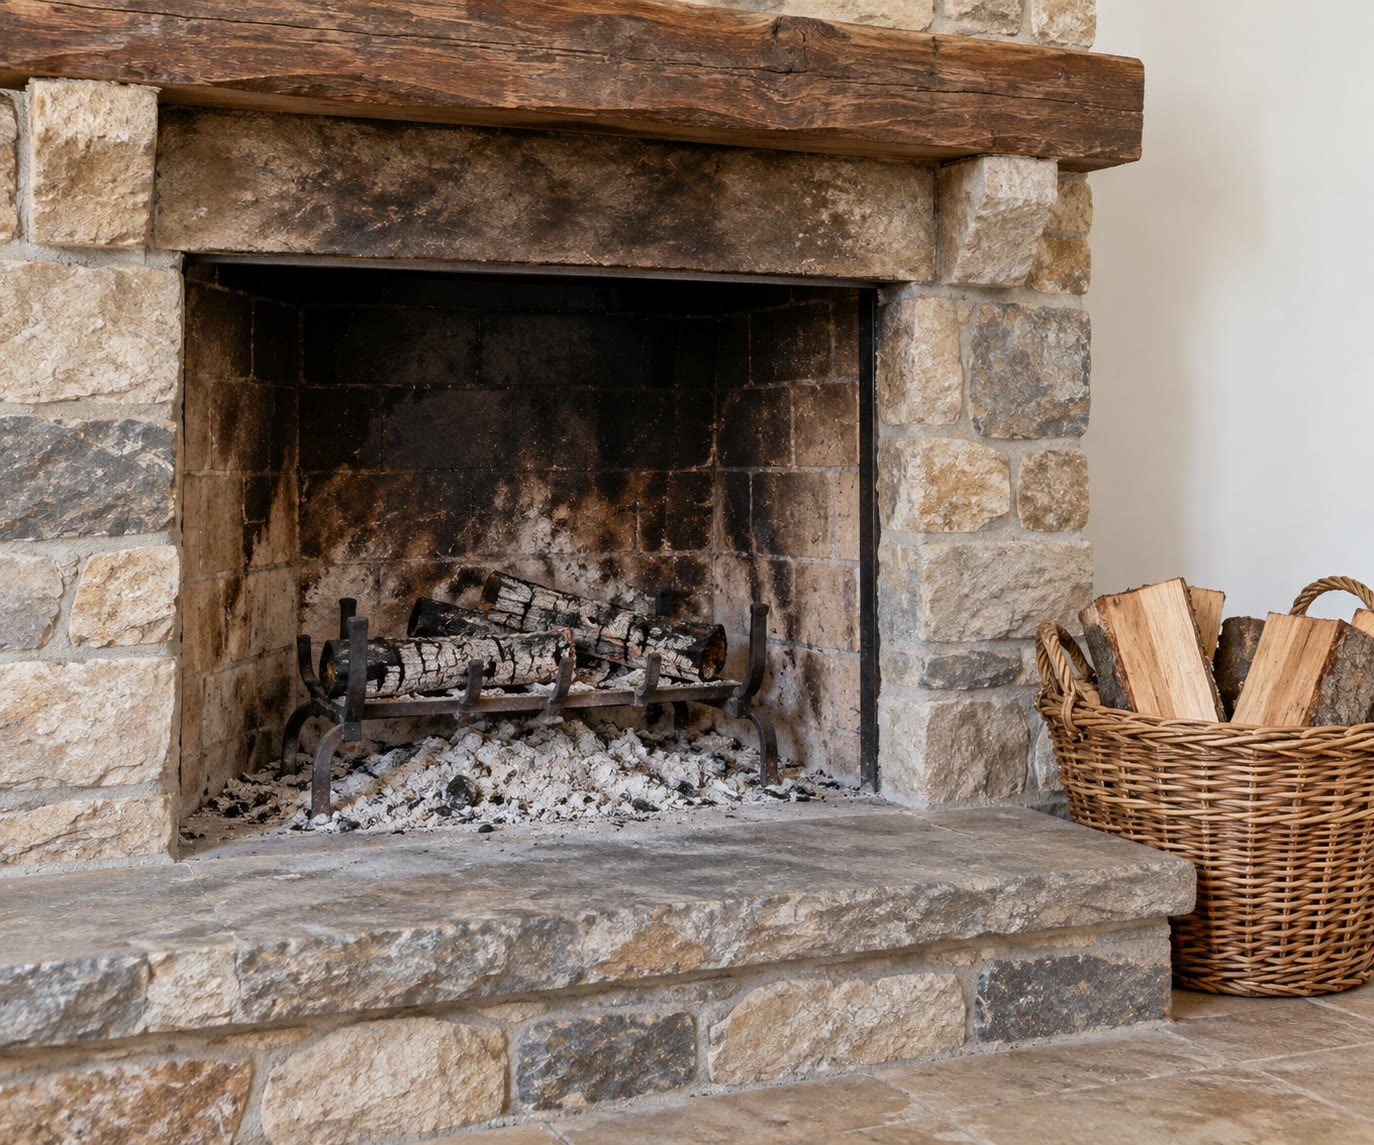
\includegraphics[width=0.5\linewidth]{images/book1/ai/g8-fireplace-ash.jpg}

{\small Perapian keesokan paginya: sedikit abu adalah satu-satunya yang
tersisa dari kayu-kayu gelondongan itu.}
\end{omfigure}

\section{Massa itu kekal}

\begin{inthelab}[Menimbang reaksi dalam labu tertutup]
Guru menuangkan sedikit cuka ke dalam sebuah labu, dan soda kue ke dalam
balon yang dipasang menutupi lehernya, lalu meletakkan semuanya di atas
neraca: \qty{212.4}{g}. Balon diangkat sehingga soda kue jatuh ke dalam
cuka: \omterm{def:g6:pure-substances-and-mixtures:mixture}{campurannya} berdesis dan balon menggembung oleh gas yang
terbentuk. Neraca tetap menunjukkan \qty{212.4}{g}. Reaksi yang sama
dalam labu terbuka, tanpa balon, ``kehilangan'' massa: gasnya lolos ke
ruangan.
\end{inthelab}

\begin{omfigure}
\begin{tikzpicture}[font=\small, scale=1.15]
  % closed flask
  \pic[transform shape] at (0,0) {balance};
  \pic[transform shape] at (0,0.8) {erlenmeyer={0.25}{omWater!80}};
  \fill[red!55, draw=red!60!black] (0,4.05) ellipse (0.5 and 0.62);
  \fill[red!55] (-0.3,3.45) rectangle (0.3,3.6);
  \node[anchor=north, align=center] at (0,-0.1) {tertutup: gasnya tetap\\ di dalam balon};
  \node[anchor=west, font=\footnotesize] at (1.25,0.3) {\qty{212.4}{g}};
  % open flask
  \pic[transform shape] at (4,0) {balance};
  \pic[transform shape] at (4,0.8) {erlenmeyer={0.25}{omWater!80}};
  \foreach \y in {3.6,3.95,4.3} \draw[->, black!45, decorate,
    decoration={snake, amplitude=0.6pt, segment length=4pt}] (4,\y) -- (4,\y+0.3);
  \node[anchor=north, align=center] at (4,-0.1) {terbuka: gasnya lolos,\\ angka neraca turun};
  \node[anchor=west, font=\footnotesize] at (5.25,0.3) {\qty{211.9}{g}};
\end{tikzpicture}

{\small Reaksi yang sama, ditimbang. Dalam labu tertutup massanya tidak
berubah; dalam labu terbuka gasnya keluar dan neraca menunjukkan angka
yang lebih kecil.}
\end{omfigure}

\begin{definition}[Kekekalan massa]\label{def:g8:balanced-equations:conservation}
Yang disebut \emph{kekekalan massa}\index{kekekalan massa} adalah hukum
yang menyatakan bahwa dalam \omterm{def:g7:chemical-reactions:reaction}{reaksi kimia}, massa total produk yang
terbentuk sama dengan massa total \omterm{def:g7:chemical-reactions:reactant}{pereaksi} yang terpakai. Tidak ada yang
hilang dan tidak ada yang diciptakan; materi hanya berubah bentuk.
\end{definition}

\begin{example}[Kayu gelondongan, ditimbang dengan benar]\label{ex:g8:balanced-equations:log}
Seandainya kayu yang \omterm{def:g4:what-a-fire-needs:burning}{terbakar} dan oksigen yang diambilnya dari \omterm{def:g4:air-a-mixture-of-gases:air}{udara}
dapat ditimbang sebelumnya, lalu abu, karbon dioksida, dan uap air
ditimbang sesudahnya, kedua jumlah itu akan sama. Abunya ringan karena
sebagian besar produknya berupa gas yang naik melalui cerobong.
\end{example}

\begin{history}[Lavoisier menimbang segalanya, 1770-an--1789]
Antoine-Laurent Lavoisier menjadikan kebiasaan untuk menimbang setiap
zat sebelum dan sesudah setiap reaksi, dalam bejana tertutup rapat agar
tidak ada gas yang dapat keluar atau masuk. Ia menunjukkan bahwa logam
bertambah massanya ketika berkarat atau \omterm{def:g4:what-a-fire-needs:burning}{terbakar}, karena mengambil
sesuatu dari \omterm{def:g4:air-a-mixture-of-gases:air}{udara} --- oksigen, yang ia namai --- dan pada tahun 1789
menyatakan bahwa dalam reaksi tidak ada yang diciptakan dan tidak ada
yang hilang. Istrinya, Marie-Anne Paulze Lavoisier, bekerja di
sampingnya, mencatat percobaan-percobaannya, dan menggambar
peralatannya untuk bukunya.
\end{history}

\begin{omfigure}
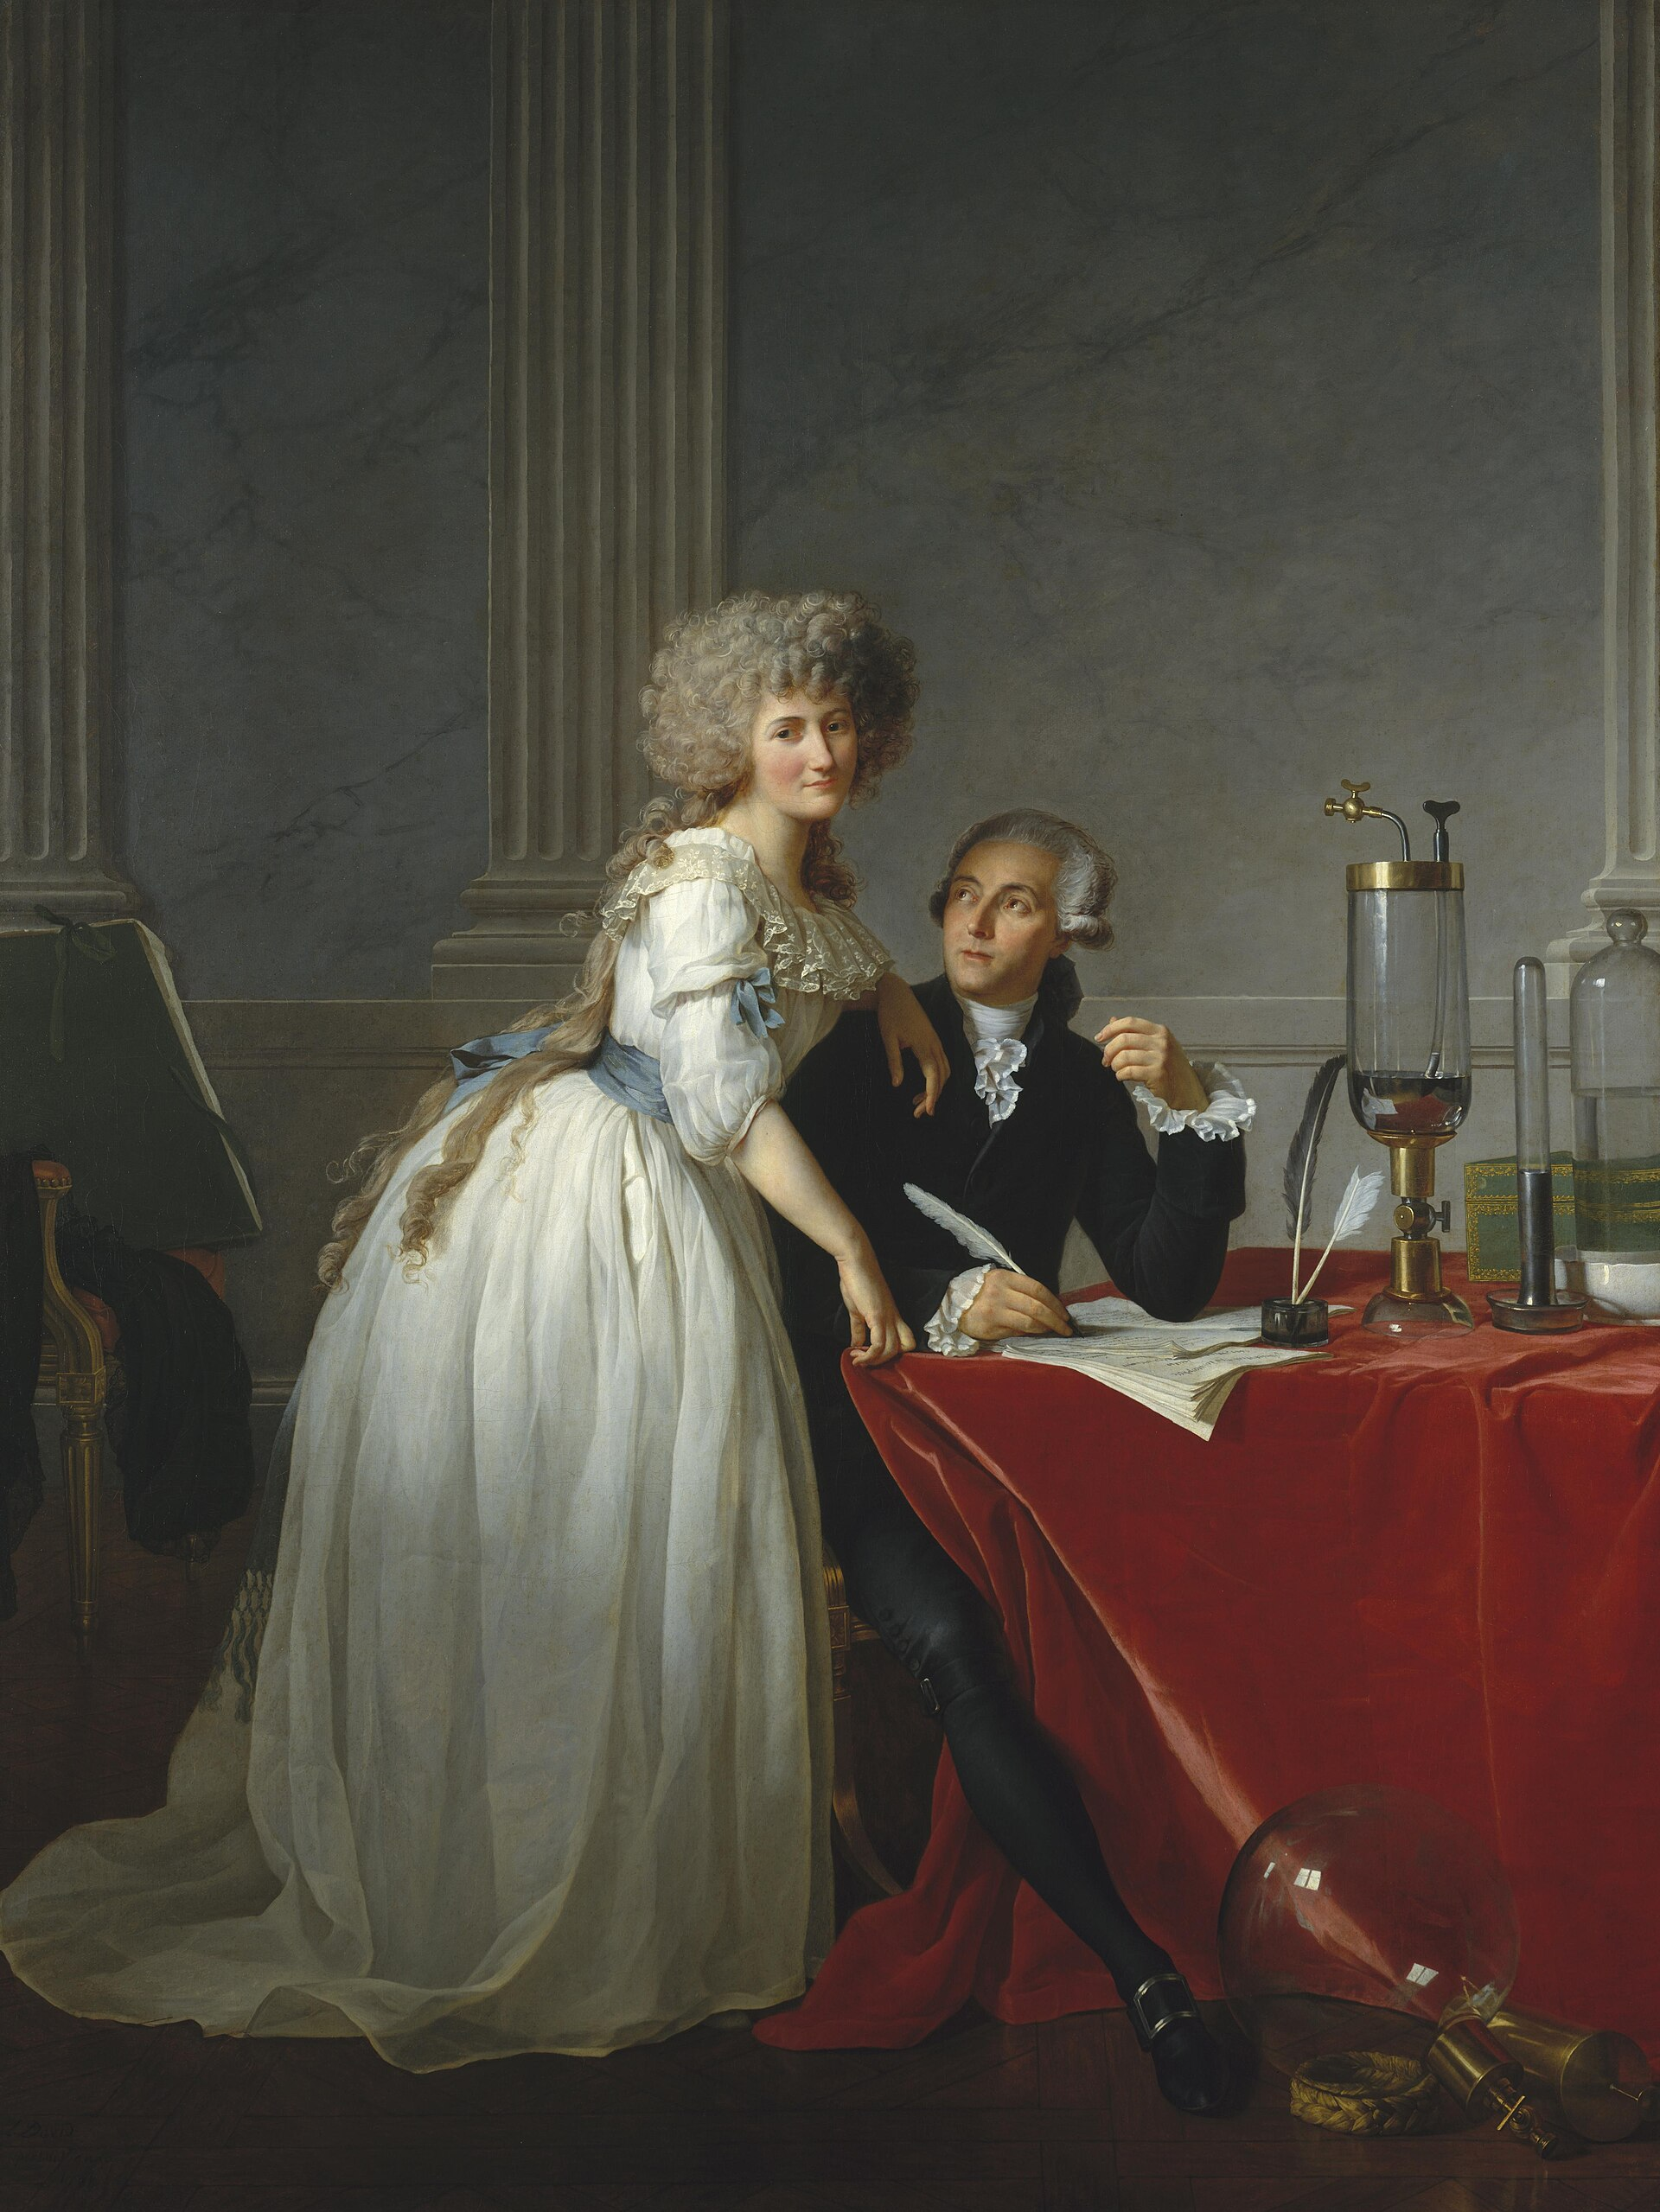
\includegraphics[width=0.3\linewidth]{images/book1/lavoisier.jpg}

{\small Antoine-Laurent Lavoisier dan Marie-Anne Paulze Lavoisier, karya
Jacques-Louis David, 1788.}
\end{omfigure}

\section{Mengapa massa kekal}

\begin{proposition}[Atom kekal, maka massa kekal]\label{prop:g8:balanced-equations:why}
Dalam reaksi, \omterm{def:g7:atoms-and-molecules:atom}{atom-atom} hanya ditata ulang: setiap \omterm{def:g7:atoms-and-molecules:atom}{atom} \omterm{def:g7:chemical-reactions:reactant}{pereaksi}
ditemukan lagi dalam produk. Setiap \omterm{def:g7:atoms-and-molecules:atom}{atom} tetap memiliki massanya
sendiri. Karena itu massa totalnya tidak dapat berubah.
\end{proposition}

\begin{example}[Besi yang bertambah massanya]\label{ex:g8:balanced-equations:iron}
Wol baja yang dibakar di atas neraca dalam cawan terbuka menjadi lebih
berat: \omterm{def:g7:atoms-and-molecules:atom}{atom-atom} besi telah bergabung dengan \omterm{def:g7:atoms-and-molecules:atom}{atom-atom} oksigen yang
diambil dari \omterm{def:g4:air-a-mixture-of-gases:air}{udara}, dan oksida besi yang terbentuk seberat besi
ditambah oksigen itu. Jika dibakar dalam stoples \omterm{def:g4:air-a-mixture-of-gases:air}{udara} yang tertutup
rapat di atas neraca, massa keseluruhannya tidak berubah: oksigen itu
sudah berada di dalam stoples.
\end{example}

\section{Persamaan reaksi}

\begin{definition}[Persamaan reaksi]\label{def:g8:balanced-equations:equation}
Sebuah \emph{persamaan reaksi}\index{persamaan reaksi} menuliskan reaksi
dengan rumus-rumus: rumus \omterm{def:g7:chemical-reactions:reactant}{pereaksi} di kiri, dihubungkan dengan $+$,
sebuah anak panah, dan rumus produk di kanan. Setiap rumus boleh
diawali sebuah angka. Persamaan itu disebut
\emph{persamaan setara}\index{persamaan setara} jika setiap jenis \omterm{def:g7:atoms-and-molecules:atom}{atom}
muncul sama banyak di kedua ruas.
\end{definition}

\begin{definition}[Koefisien stoikiometri]\label{def:g8:balanced-equations:coefficient}
Angka yang ditulis di depan rumus dalam sebuah persamaan adalah
\emph{koefisien stoikiometri}\index{koefisien stoikiometri} rumus itu:
angka itu menghitung \omterm{def:g7:atoms-and-molecules:molecule}{molekul} (atau partikel lain) spesies itu yang ikut
serta. Koefisien 1 tidak ditulis.
\end{definition}

\begin{notation}[Lambang wujud]\label{not:g8:balanced-equations:states}
Huruf dalam tanda kurung sesudah rumus dapat menyatakan wujudnya: (s)
padat, (l) cair, (g) gas. Jadi \ce{H2O(l)} adalah air cair dan
\ce{H2O(g)} uap air.
\end{notation}

\begin{example}[Membaca persamaan]\label{ex:g8:balanced-equations:read}
\[
  \ce{CH4(g) + 2O2(g) -> CO2(g) + 2H2O(l)}
\]
dibaca: satu \omterm{def:g7:atoms-and-molecules:molecule}{molekul} metana dan dua \omterm{def:g7:atoms-and-molecules:molecule}{molekul} oksigen bereaksi
menghasilkan satu \omterm{def:g7:atoms-and-molecules:molecule}{molekul} karbon dioksida dan dua \omterm{def:g7:atoms-and-molecules:molecule}{molekul} air. Kiri:
1 C, 4 H, 4 O. Kanan: 1 C, 4 H, $2 + 2 = 4$ O. Persamaan itu setara.
\end{example}

\begin{omfigure}
\begin{tikzpicture}[font=\small]
  \begin{scope}[every node/.style={font=\Large, inner sep=2pt}]
    \node (a) at (0,0) {\ce{CH4}};
    \node (p1) at (0.95,0) {$+$};
    \node (b) at (1.9,0) {\ce{2O2}};
    \node (arr) at (3.35,0) {$\longrightarrow$};
    \node (c) at (4.8,0) {\ce{CO2}};
    \node (p2) at (5.75,0) {$+$};
    \node (d) at (6.8,0) {\ce{2H2O}};
  \end{scope}
  \draw[thick, omDef] ([yshift=-2pt]a.south west) -- ++(0,-0.15) -| ([yshift=-2pt]b.south east);
  \node[below=8pt, text=black] at ($(a.south)!0.5!(b.south)$) {pereaksi};
  \draw[thick, omProp] ([yshift=-2pt]c.south west) -- ++(0,-0.15) -| ([yshift=-2pt]d.south east);
  \node[below=8pt, text=black] at ($(c.south)!0.5!(d.south)$) {produk};
  \node[above=6pt of arr, font=\small] {``bereaksi menghasilkan''};
  \node[anchor=north west, align=left, draw=black!35, rounded corners=2pt,
    font=\small, inner sep=4pt] at (-0.3,-1.25)
    {Pada \ce{2O2}: angka 2 besar di depan adalah \textbf{koefisien} (dua molekul);\\
     angka 2 kecil di bawah garis adalah \textbf{angka indeks} (dua atom dalam setiap molekul).};
\end{tikzpicture}

{\small Bagian-bagian sebuah \omterm{def:g8:balanced-equations:equation}{persamaan reaksi}.}
\end{omfigure}

\section{Menyetarakan persamaan}

\begin{method}[Menyetarakan persamaan]\label{met:g8:balanced-equations:balance}
\begin{enumerate}
  \item Tuliskan rumus \omterm{def:g7:chemical-reactions:reactant}{pereaksi} dan produk yang benar. Jangan pernah
        mengubah rumus sesudahnya: mengubah \ce{H2O} menjadi \ce{H2O2}
        akan menggambarkan zat yang lain.
  \item Hitung \omterm{def:g7:atoms-and-molecules:atom}{atom} setiap jenis di setiap ruas.
  \item Setarakan satu jenis \omterm{def:g7:atoms-and-molecules:atom}{atom} demi satu dengan koefisien, dimulai
        dari \omterm{def:g7:atoms-and-molecules:atom}{atom} yang hanya muncul dalam satu rumus di setiap ruas;
        biarkan hidrogen dan oksigen sampai terakhir.
  \item Hitung lagi; ulangi sampai setiap jenis \omterm{def:g7:atoms-and-molecules:atom}{atom} setara.
  \item Pakailah bilangan bulat terkecil.
\end{enumerate}
\end{method}

\begin{example}[Hidrogen dan oksigen]\label{ex:g8:balanced-equations:water}
Belum setara: \ce{H2 + O2 -> H2O} % ce-unbalanced-ok (the skeleton)
memiliki 2 O di kiri, 1 di kanan. Taruh 2 di depan \ce{H2O}: sekarang
ada 4 H di kanan, jadi 2 di depan \ce{H2}:
\[
  \ce{2H2 + O2 -> 2H2O}.
\]
Periksa: 4 H dan 2 O di setiap ruas.
\end{example}

\begin{example}[Besi terbakar dalam oksigen]\label{ex:g8:balanced-equations:iron-oxide}
Besi dan oksigen menghasilkan oksida besi \ce{Fe2O3}. Oksigen: 2 di kiri,
3 di kanan; bilangan persekutuan terkecilnya 6, jadi 3 \ce{O2} dan 2
\ce{Fe2O3}. Lalu ada 4 Fe di kanan, jadi 4 Fe di kiri:
\[
  \ce{4Fe + 3O2 -> 2Fe2O3}.
\]
\end{example}

\begin{omfigure}
\begin{tikzpicture}[font=\small]
  % 2 H2
  \foreach \y in {0.45,-0.45} {
    \node[aH] (a) at (0,\y) {}; \node[aH] (b) at (0.45,\y) {};
    \begin{scope}[on background layer]\draw[bond] (a.center) -- (b.center);\end{scope}}
  \node at (1.05,0) {$+$};
  \node[aO] (a) at (1.6,0) {}; \node[aO] (b) at (2.25,0) {};
  \begin{scope}[on background layer]
    \draw[bond, line width=1.1pt] ([yshift=1.6pt]a.center) -- ([yshift=1.6pt]b.center);
    \draw[bond, line width=1.1pt] ([yshift=-1.6pt]a.center) -- ([yshift=-1.6pt]b.center);
  \end{scope}
  \draw[->, thick, omProp] (2.9,0) -- (3.9,0);
  \foreach \y in {0.5,-0.5} {
    \node[aO] (o) at (4.9,\y+0.12) {};
    \node[aH] (p) at (4.35,\y-0.28) {}; \node[aH] (q) at (5.45,\y-0.28) {};
    \begin{scope}[on background layer]
      \draw[bond] (o.center) -- (p.center); \draw[bond] (o.center) -- (q.center);
    \end{scope}}
  \node[align=center, font=\footnotesize] at (1.1,-1.35) {4 H, 2 O};
  \node[align=center, font=\footnotesize] at (4.9,-1.35) {4 H, 2 O};
  \node[font=\small] at (2.7,-2.0) {\ce{2H2 + O2 -> 2H2O}};
\end{tikzpicture}

{\small \omterm{def:g8:balanced-equations:equation}{Persamaan setara} \omterm{def:g4:what-a-fire-needs:burning}{pembakaran} hidrogen, digambar dengan model: dua
\omterm{def:g7:atoms-and-molecules:molecule}{molekul} hidrogen dan satu \omterm{def:g7:atoms-and-molecules:molecule}{molekul} oksigen menghasilkan dua \omterm{def:g7:atoms-and-molecules:molecule}{molekul} air.}
\end{omfigure}

\section{Membaca persamaan dalam molekul}


\begin{proposition}[Apa yang dikatakan persamaan setara]\label{prop:g8:balanced-equations:molecules}
Koefisien-koefisien \omterm{def:g8:balanced-equations:equation}{persamaan setara} menyatakan perbandingan
partikel-partikel yang bereaksi dan terbentuk. Jika persamaannya
\ce{2H2 + O2 -> 2H2O}, maka 200 \omterm{def:g7:atoms-and-molecules:molecule}{molekul} hidrogen bereaksi dengan 100
\omterm{def:g7:atoms-and-molecules:molecule}{molekul} oksigen menghasilkan 200 \omterm{def:g7:atoms-and-molecules:molecule}{molekul} air; sejuta \omterm{def:g7:atoms-and-molecules:molecule}{molekul} oksigen
memerlukan dua juta \omterm{def:g7:atoms-and-molecules:molecule}{molekul} hidrogen.
\end{proposition}

\begin{example}[Propana di kompor kemah]\label{ex:g8:balanced-equations:propane}
Propana, \ce{C3H8}, \omterm{def:g4:what-a-fire-needs:burning}{terbakar} dalam oksigen menghasilkan karbon dioksida
dan air. Karbon dulu: 3 C, jadi 3 \ce{CO2}. Hidrogen: 8 H, jadi 4
\ce{H2O}. Oksigen di kanan: $3 \times 2 + 4 = 10$ O, jadi 5 \ce{O2}:
\[
  \ce{C3H8 + 5O2 -> 3CO2 + 4H2O}.
\]
Setiap \omterm{def:g7:atoms-and-molecules:molecule}{molekul} propana memerlukan lima \omterm{def:g7:atoms-and-molecules:molecule}{molekul} oksigen.
\end{example}

\section{Latihan}

\begin{exercise}[$\star$]\label{exo:g8:balanced-equations:1}
Nyatakan hukum \omterm{def:g8:balanced-equations:conservation}{kekekalan massa}.
\end{exercise}

\begin{exercise}[$\star$]\label{exo:g8:balanced-equations:2}
Pada \ce{3CO2}, berapa \omterm{def:g8:balanced-equations:coefficient}{koefisien stoikiometrinya}? Berapa \omterm{def:g7:atoms-and-molecules:atom}{atom} karbon
dan berapa \omterm{def:g7:atoms-and-molecules:atom}{atom} oksigen yang dinyatakannya?
\end{exercise}

\begin{exercise}[$\star$]\label{exo:g8:balanced-equations:3}
Apakah \ce{C + O2 -> CO2} setara? Hitung \omterm{def:g7:atoms-and-molecules:atom}{atom-atomnya} untuk memeriksa.
\end{exercise}

\begin{exercise}[$\star$]\label{exo:g8:balanced-equations:4}
Setarakan \ce{Mg + O2 -> MgO}. % ce-unbalanced-ok (to balance)
\end{exercise}

\begin{exercise}[$\star\star$]\label{exo:g8:balanced-equations:5}
Setarakan \ce{N2 + H2 -> NH3}, reaksi pembuatan amonia. % ce-unbalanced-ok (to balance)
\end{exercise}

\begin{exercise}[$\star\star$]\label{exo:g8:balanced-equations:6}
Sebanyak \qty{12}{g} karbon \omterm{def:g4:what-a-fire-needs:burning}{terbakar} sempurna dan membentuk
\qty{44}{g} karbon dioksida. Berapa massa oksigen yang terpakai?
\end{exercise}

\begin{exercise}[$\star\star$]\label{exo:g8:balanced-equations:7}
Lihatlah gambar dua labu di atas neraca. Mengapa angka neraca untuk labu
yang terbuka turun? Apakah ada massa yang dimusnahkan?
\end{exercise}

\begin{exercise}[$\star\star$]\label{exo:g8:balanced-equations:8}
Setarakan \ce{CH4 + O2 -> CO2 + H2O} langkah demi langkah, sambil % ce-unbalanced-ok (to balance)
menyebutkan \omterm{def:g7:atoms-and-molecules:atom}{atom} mana yang kamu setarakan pada setiap langkah.
\end{exercise}

\begin{exercise}[$\star\star$]\label{exo:g8:balanced-equations:9}
Seorang siswa menyetarakan \ce{H2 + O2 -> H2O} dengan menulis \ce{H2 + O2 -> H2O2}. % ce-unbalanced-ok (the student's start)
Mengapa cara ini salah?
\end{exercise}

\begin{exercise}[$\star\star$]\label{exo:g8:balanced-equations:10}
Dengan \ce{C3H8 + 5O2 -> 3CO2 + 4H2O}, berapa \omterm{def:g7:atoms-and-molecules:molecule}{molekul} oksigen yang
diperlukan untuk membakar 20 \omterm{def:g7:atoms-and-molecules:molecule}{molekul} propana? Berapa \omterm{def:g7:atoms-and-molecules:molecule}{molekul} air yang
terbentuk?
\end{exercise}

\begin{exercise}[$\star\star\star$]\label{exo:g8:balanced-equations:11}
Setarakan \ce{C2H6 + O2 -> CO2 + H2O}, \omterm{def:g4:what-a-fire-needs:burning}{pembakaran} etana. (Petunjuk: coba % ce-unbalanced-ok (to balance)
gandakan etananya.)
\end{exercise}

\begin{exercise}[$\star\star\star$]\label{exo:g8:balanced-equations:12}
Sebatang lilin \qty{20.0}{g} menyala di dalam kotak kaca tertutup rapat
yang penuh \omterm{def:g4:air-a-mixture-of-gases:air}{udara}, yang diletakkan di atas neraca yang menunjukkan
\qty{850.0}{g} seluruhnya. Ketika nyalanya padam, lilin itu tinggal
\qty{19.6}{g}. Berapa angka yang ditunjukkan neraca? Jelaskan.
\end{exercise}

\section{Soal: Wol Baja dalam Stoples Tertutup}

\begin{problem}[{Soal akhir pekan --- besi yang terbakar, neraca yang tidak
bergeming, dan oksigen yang diambil dari udara}]
\label{pb:g8:balanced-equations:1}
Di laboratorium, seorang guru membakar wol baja, yang hampir berupa besi
murni, dengan dua cara. Pertama, segumpal wol baja dibakar dalam cawan
terbuka di atas neraca: angkanya naik. Lalu segumpal wol baja
\qty{0.28}{g} dibakar, dinyalakan dengan percikan listrik, di dalam
stoples \omterm{def:g4:air-a-mixture-of-gases:air}{udara} yang tertutup di atas neraca: angkanya tidak berubah.
Stoples itu berisi sekitar \qty{0.5}{g} oksigen. Besi yang \omterm{def:g4:what-a-fire-needs:burning}{terbakar}
dalam oksigen membentuk oksida besi \ce{Fe2O3}; dengan oksigen yang
lebih sedikit, besi juga dapat membentuk \ce{Fe3O4}.

\medskip
\noindent\textbf{Bagian I --- Dua penimbangan.}
\begin{enumerate}
  \item Dalam cawan terbuka, massanya naik. Dari mana massa tambahan itu
        berasal?
  \item Dalam stoples tertutup, massanya tidak berubah. Jelaskan.
  \item Nyatakan hukum yang digambarkan oleh kedua penimbangan ini.
\end{enumerate}

\medskip
\noindent\textbf{Bagian II --- Dua persamaan.}
\begin{enumerate}[resume]
  \item Setarakan persamaan \ce{Fe + O2 -> Fe2O3}. % ce-unbalanced-ok (to balance)
  \item Setarakan persamaan \ce{Fe + O2 -> Fe3O4}. % ce-unbalanced-ok (to balance)
  \item Periksa persamaan pertama dengan menghitung \omterm{def:g7:atoms-and-molecules:atom}{atom} setiap jenis di
        setiap ruas.
  \item Menurut persamaan pertama, berapa \omterm{def:g7:atoms-and-molecules:molecule}{molekul} oksigen yang bereaksi
        dengan 400 \omterm{def:g7:atoms-and-molecules:atom}{atom} besi?
\end{enumerate}

\medskip
\noindent\textbf{Bagian III --- Massa.}
Dalam \ce{Fe2O3}, setiap \qty{7}{g} besi bergabung dengan \qty{3}{g}
oksigen. Gumpalan wol baja \qty{0.28}{g} itu \omterm{def:g4:what-a-fire-needs:burning}{terbakar} sempurna menjadi
\ce{Fe2O3}.
\begin{enumerate}[resume]
  \item Berapa massa oksigen yang bergabung dengan \qty{0.28}{g} besi?
  \item Berapa massa oksida besi yang terbentuk?
  \item Apakah oksigen di dalam stoples cukup? Jelaskan.
  \item Stoples dibuka setelah dingin, dan \omterm{def:g4:air-a-mixture-of-gases:air}{udara} menyerbu masuk. Jelaskan
        mengapa, dan katakan bagaimana angka neraca lalu berubah.
  \item Hitung massa oksigen yang diambil oleh wol baja yang \omterm{def:g4:what-a-fire-needs:burning}{terbakar} dari
        \omterm{def:g4:air-a-mixture-of-gases:air}{udara} di dalam stoples.
\end{enumerate}
\end{problem}
